\chapter{Admin Web Interface}
This chapter goes into details about the design and implementation of the website used to administrate Media-Online Management (MOM).

\section{Design}\fixme{Her er sikkert en masse 'we' som kan undværes}
%Interface Design
%What you can do from the website, and how
As mentioned in the overview, see subsection \vref{section:momswebsite}, we know what the website is required to do for the system.
These requirements made the basis for deciding what pages should be created and what each page's functionality should be. During the designing of the website we aimed to fit all relevant information into each page.\\
All pages have been designed on the blackboards, where we discovered inconsistencies, new navigation paths and learn about how concepts such as rules should be implemented.\\
Next is a short overview of what pages were designed and their purposes.\\
\\
\textbf{Dashboard} is used to get a quick overview of relevant data. The overview is customizable so that each parent can decide what information is most relevant for them.\\
\\
\textbf{Devices} is used to get an overview of which controllers and tags is registered within their MOM system. It also is the only way to navigate to the Add Tag/Controller and Details Tag/Controller pages.\\
From this page it is also possible to deactivate a tag, meaning the owner of that tag, can no longer log in with it.\\
\\
\textbf{Devices - Details Controller} is used to display, delete and change information about a controller. A user can only access controllers that is registered to his system.\\
\\
\textbf{Devices - Details Tag} is used to display, delete and change information about a tag. A user can only access tags that is registered to his system.\\
\\
\textbf{Devices - Add Controller} is used to add controllers to the user's system. In order to add a controller the user must add a unique key found on the controller, this is then checked towards a database of available keys.\\
However we have not currently implemented this way of validation, but it would be the right way to go in order to commercialize the system and ensure security for our users.\\
\\
\textbf{Devices - Add Tag} is like Add Controller, except with tags. Also in order to register a tag, a user must be dedicated to this tag. The one registering a tag, will be meet by a list of current users in the system. This means that in order to apply a tag, one must first create a user, then register a tag.\\
\\
\textbf{Users} is used to get an overview of users in one's system. It is also used to navigate to Create User and User Details.\\
\\
\textbf{Users - User Details} is for viewing details about a user. It is also used to change information about a user, however it is only possible to change information, if your user is of a manager-role, or if you are the owner of that profile.\\
\\
\textbf{Users - Create User} is as the name suggests, used for creating a user. We are making the system ready for children to login to the system already now. We do not have any feature that requires the children to log in to the system as of yet, but a feature might utilize this later on.\\
\\
\textbf{Users - Chores} is used to get an overview of available chores, and for easy rewarding of already created chores. When a chore is done, the parent should go to this site, and simply select a child and press a button to give them the assigned reward of the chore.\\
Chores will also have a subsite for creating chores.\\
\\
\textbf{Users - Rules} is where parents can get an overview of rules and create them for their system. We have taken great care to help users in creating rules, by making a step by step procedure. Starting with making the user choose what sort of action they want to achieve and thereafter choose the sort of condition they want to set, since actions only match certain conditions. This should limit some of the confusion about the rules. For more information about rules, actions and conditions see subsection \vref{sec:rule}.\\
\\
\textbf{Users - Permissions} is designed for an easier way to think of rules, in relation to what devices which child is allowed to use in which time slots of the days.\\
We decided to create this permissions page, because permissions is an essential part of even the smallest of systems. This tool gives the parents an easy way to limit their child’s usage, by deciding devices can not be turned on after a certain time.\\
\\
\textbf{Graf} page is intended for viewing statistics, such as how much have a controller been active, how is a users usage of media divided and so forth.\\
\\
\textbf{Calendar} has two purposes. It serves as a graphical presentation of rules, in the sense that it shows when a rule will apply, and to what user.\\
It also serves to provide a shortcut to create rules, from other calendars. For example, if the user has a Google calendar, that have been registered to the system, they can simply click that event and the system will start creating a rule with a condition corresponding to the calendar events configuration.\\
\\
Every page have been explained and in the next section the navigation is explained.
%Navigation
\subsection{Navigation}
When the user has logged in, they are navigated to the dashboard. From here and every other page they can navigate to the main pages: Dashboard, Devices, Users, Permissions, Rules, Chores, Graf and Calendar, see figure \ref{fig:navigationOfWebsite}.\\
We decided to keep our navigation as simple as possible. In the design there is 5 head menus, Dashboard, Devices, Users, Graf and Calendar. Meaning Permissions, Rules and Chores are sub-menus and these are all listed under Users.\\


\begin{figure}[htbp]
	\centering
		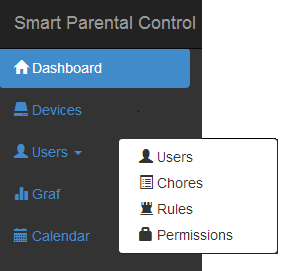
\includegraphics[width=0.50\textwidth]{images/navigationOfWebsite.png}
	\caption{Website Navigation}
	\label{fig:navigationOfWebsite}
\end{figure}


We also designed the system such that no other menu or functionality is any more than 2 clicks away, every add or detail function can be accessed directly from one of the head menus.\\

\subsection{Color Scheme and Layout Design}
%Color Schemes
%Bootstrap and other inspiration sources
Our color scheme and layout design was inspired by both bootstrap and a website which utilizes bootstrap, called SB Admin\citep{sbadmin}. We have used a standard bootstrap color scheme, and added in a little blue, we wanted to keep the colors simple but no further thought was put into it.\\
The most of the design is based on standard tools from bootstrap. With exception of the table sorter functionality. Which is a JQuery tool that allows for sorting of tables.\\
We chose to use bootstrap since it gives an okay design and it is easy to implement prototypes in bootstrap.	


\section{Implementation}
The previous section explained what each page should do, and in some detail how from the users viewpoint.

The implementation itself of the web-pages is not very interesting since they are based on a simple format of inputting the required information and submitting it to the server.\\
A few of the functionalists are however a bit more advanced. Two of these are toggling activity of a user and the page for users.\\

\subsection{Toggling Activity}
%AJAX
%PHP

Under the page Devices, the overview of tags and controllers can be seen. But this is also were the activity of a user can be toggled.

\begin{figure}[htbp]
	\centering
		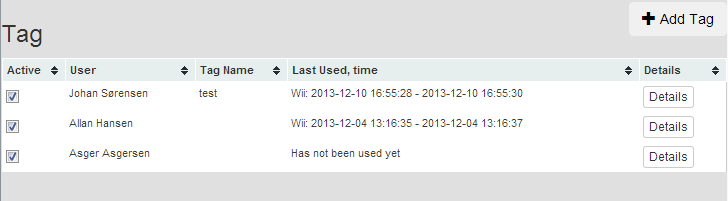
\includegraphics[width=1.00\textwidth]{images/tagOverview.PNG}
	\caption{Tag Overview}
	\label{fig:tagOverview}
\end{figure}

This is done by pressing the checkbox in the left side of the tags overview, see figure \ref{fig:tagOverview}. When this is pressed it activates an AJAX call that makes a http request to the PHP page \texttt{setActiveTag.php}. That PHP page then makes a query to the database in order to set the \texttt{active} status of a tag in the system, see figure \ref{fig:flowChartTagActivity}. Resulting in the user no longer being able to use said tag. If it is pressed again the opposite happens and the user can again use said tag.


\begin{figure}[htbp]
	\centering
		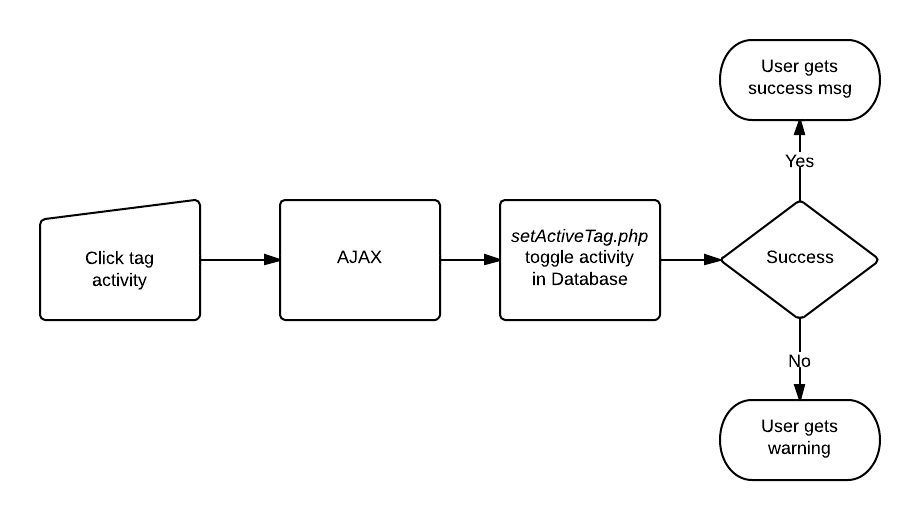
\includegraphics[width=0.75\textwidth]{images/flowChartTagActivity.png}
	\caption{Flowchart for Toggling Activity}
	\label{fig:flowChartTagActivity}
\end{figure}


\subsection{The Rules Page}
%Database communication
%JQuery
